\section*{Introduction}

The analysis of magnetic field data is a key component in geophysical investigations, offering valuable information about subsurface structures and geological variations \citep{Blakely1988}. Among the techniques available for processing such data, the equivalent source method is particularly useful. Based on principles from potential theory, this method takes advantage of the inherent non-uniqueness of potential fields by replacing observed anomalies with synthetic responses from a set of hypothetical sources. These sources are used to perform common geophysical operations such as upward and downward continuation, gridding, and reduction to the pole \citep{Dampney1969}.

This approach typically relies on a distribution of virtual sources located below the observation surface to improve numerical stability. However, its application to large-scale datasets, such as those acquired in airborne surveys,can be computationally demanding due to the high volume of data. \citet{OliveiraJunior2023} discuss this limitation and review several strategies designed to reduce computational cost. These include Column- and Row-action updates, sparsity regularization, iterative and direct deconvolution, and the Moving Window technique introduced by \citet{leao1989} and further developed by \citet{soler2021}.

In this work, we extend the equivalent source method to spherical coordinates and incorporate a gradient-boosting strategy of \citet{soler2021} also using the dual-layer method of \citet{Uppal2025} to fit booth higher- and lower-wavelength. This combination is intended to improve the efficiency and scalability of modeling magnetic data over regional to continental areas, where the curvature of the Earth must be taken into account. The method includes a windowed inversion framework with iterative refinement, adapted to the geometry of the sphere.

Equivalent source methods have traditionally been applied to problems at local and regional scales, particularly in geological mapping and mineral exploration \citep{Emilia1973, Mendonca1994, Mendonca1995, Gusp2009, Li2006, Li2020, ZhiWen2022}. However, the increasing availability of large-scale geophysical datasets and the growing interest in regional to global studies have highlighted the limitations of Cartesian formulations in these contexts. As the scale of analysis increases, the curvature of the Earth can no longer be neglected, and methods formulated in spherical coordinates become more appropriate \citep{VonFrese1981}. Despite the continued use of Cartesian-based approaches, largely due to their simpler implementation and well-established computational infrastructure \citep{Li2010, Siqueira2017, Jirigalatu2019, soler2021, takahashi2022},they tend to introduce geometric distortions over large areas, reducing the reliability of the results in spherical domains.

Spherical approaches, in contrast, are more appropriate for large-scale modeling and have been successfully used in global anomaly studies and satellite data analysis \citep{Langel1998, Kother2015}. Nonetheless, extending the equivalent source technique to a spherical geometry introduces additional mathematical and computational challenges. These include reformulating the sensitivity matrix, adapting inversion algorithms, and ensuring numerical stability in the presence of noise and uneven data coverage.

To address these issues, this study aims to develop and evaluate a spherical equivalent source method enhanced with gradient-boosting techniques. We begin by testing the method with synthetic data to assess its accuracy and numerical performance. We then analyze its behavior under conditions such as varying noise levels and non-uniform spatial sampling. The gradient-boosting algorithm is adapted to the spherical setting to ensure convergence and efficiency. Finally, we apply the method to real airborne datasets to demonstrate its practical utility and potential for integration into open-source geophysical software.

Finally, we validate the method using real airborne datasets, demonstrating its applicability to complex geological scenarios, and integrate the implementation into open-source platforms such as Harmonica and Choclo, supporting broader adoption in the geophysical community. A regular grid for regional data integration is also constructed to support visualization and future comparative analyses.


%%%%%%%%%%%%%%%%%%%%%%%%%%%%%%%%%%%%%%%%%%%%%%%%%%%%%%%%%%%%%%%%%%%%%%%%%%%%%%%
\section{Methodology}
\subsection{Magnetic field of a dipole in spherical coordinates}

Magnetic field calculations in spherical coordinates are fundamental to geophysical applications such as Earth's magnetic field modeling, mineral exploration, and analysis of airborne magnetometric surveys. These applications demand mathematical descriptions that take into account Earth's curvature, especially at regional to global scales. The spherical coordinate system provides a natural framework for such modeling by aligning with the geometry of the planet.

The mathematical formulation for calculating the magnetic field generated by dipole sources in spherical coordinates is well-established in classical works by \citet{VonFrese1981} and \citet{Langel1998}. These studies present comprehensive derivations of the magnetic field components and transformation matrices necessary for practical implementations.

In spherical coordinates, the local orthonormal basis vectors depend on three variables: the radial distance $r$, the colatitude $\theta$ (measured from the positive z-axis), and the longitude $\lambda$ (measured in the x-y plane) (see Figure~\ref{fig_coordinate_systems} a)). These unit vectors, $\hat{\mathbf{r}}$, $\hat{\boldsymbol{\theta}}$, and $\hat{\boldsymbol{\lambda}}$, are essential to describe both the positions of sources and observation points, as well as the directions of vector quantities such as the magnetic field and magnetic moment.

\begin{figure}[htb]
\centering

\includegraphics[width=1\linewidth]{figures/diagram-final.png}
\caption{Geometric configuration of the magnetic dipole field calculation. 
    \textbf{(a)} Spherical coordinate system centered at the origin, with the equivalent magnetic dipole located at point $Q$, characterized by its magnetic moment vector $\vec{\mathbf{m'}}$ (blue). The magnetic field $\vec{\mathbf{B}}$ (red) is evaluated at point $P$, and both locations have their respective local reference frames defined by the spherical basis vectors $\hat{\mathbf{r}}, \hat{\boldsymbol{\theta}}, \hat{\boldsymbol{\lambda}})$. 
    \textbf{(b)} Geodetic coordinate system illustrating the curvature of the Earth and the angular separation between source and observation points, denoted by spherical and geodetic longitudes $\phi$ and $\varphi$. The difference $\varphi - \phi$ accounts for the azimuthal angle between the two coordinate systems.}
\label{fig_coordinate_systems}
\end{figure}

Expressing the magnetic field vector in the Cartesian coordinate system, we write
\begin{equation}
   \vec{\mathbf{B}} = B_x \, \hat{\mathbf{x}} + B_y \, \hat{\mathbf{y}} + B_z \, \hat{\mathbf{z}},
\end{equation}
which is often convenient for numerical computations and for relating with global coordinate references. Similarly, the magnetic moment of the source dipole is described in a Cartesian basis:
\begin{equation}
   \vec{\mathbf{m'}} = m'_x \, \hat{\mathbf{x}'} + m'_y \, \hat{\mathbf{y}'} + m'_z \, \hat{\mathbf{z}'}.
\end{equation}

However, because both the observation and source points are located on or above a spherical Earth surface, it is more appropriate to express the magnetic moment and the magnetic field in the local spherical basis at each point. The transformation between Cartesian and spherical representations involves rotation matrices composed of direction cosines.

The magnetic field vector can be expressed as a linear transformation of the source magnetic moment via the relation
\begin{equation}
   \vec{\mathbf{B}} = \frac{\mu_0}{4\pi}
   \mathbf{\bar{\bar{H}}} \mathbf{\bar{\bar{R}}}  \vec{\mathbf{m'}}.
\end{equation}
Here, the matrix $\mathbf{\bar{\bar{R}}}$ rotates the source moment vector $\mathbf{\vec{\mathbf{m'}}}$ from the source's local coordinate system to the observation point's local frame:
\begin{equation}
   \vec{\mathbf{m}} = \mathbf{\bar{\bar{R}}}\vec{\mathbf{m'}}.
\end{equation}

The rotation matrix $\mathbf{\bar{\bar{R}}}$ consists of the direction cosines $\delta_{xy'}$, which quantify the angular relationship between the unit vectors of the two local spherical bases:
\begin{equation}
\mathbf{\bar{\bar{R}}}=
    \begin{vmatrix}
\delta_{rr'} & \delta_{r\theta'} & \delta_{r\lambda'} \\
\delta_{\theta r'} & \delta_{\theta \theta'} & \delta_{\theta \lambda'} \\
\delta_{\lambda r'} & \delta_{\lambda \theta'} & \delta_{\lambda \lambda'}
    \end{vmatrix}.
\end{equation}
This matrix ensures that the vector components are consistently compared and combined across different local reference frames.

The quantities $\delta_{xy'}$ denote the direction cosines between the local spherical unit vectors at the observation point $P$ and the source point $Q$, as listed in Table~\ref{tab:dircos}. These terms encode the angular relationships between coordinate bases at different locations and are functions of the colatitude and longitude differences.

\begin{table}[h]
\centering
\caption{Expressions for direction cosines in spherical coordinates.}
\label{tab:dircos}
\begin{tabular}{ll}
\hline
\textbf{Variable} & \textbf{Expression} \\
\hline
$\delta_{rr'}$   & $\cos \theta \cos \theta' + \sin \theta \sin \theta' \cos(\phi - \phi')$ \\
$\delta_{r\theta'}$ & $-\cos \theta \sin \theta' + \sin \theta \cos \theta' \cos(\phi - \phi')$ \\
$\delta_{r\phi'}$   & $\sin \theta \sin(\phi - \phi')$ \\
$\delta_{\theta r'}$ & $-\sin \theta' \cos \theta + \cos \theta' \sin \theta \cos(\phi - \phi')$ \\
$\delta_{\theta \theta'}$ & $\sin \theta \sin \theta' + \cos \theta \cos \theta' \cos(\phi - \phi')$ \\
$\delta_{\theta \phi'}$ & $\cos \theta \sin(\phi - \phi')$ \\
$\delta_{\phi r'}$ & $-\sin \theta' \sin(\phi - \phi')$ \\
$\delta_{\phi \theta'}$ & $-\cos \theta' \sin(\phi - \phi')$ \\
$\delta_{\phi \phi'}$ & $\cos(\phi - \phi')$ \\
\hline
\end{tabular}
\end{table}



The kernel matrix $\mathbf{\bar{\bar{H}}}$ encapsulates the physical laws governing the magnetic field produced by a dipole in spherical coordinates and is defined as:
\begin{equation}
\mathbf{\bar{\bar{H}}} = 
    \begin{vmatrix}
H_{11} & H_{12} & H_{13}\\
H_{21} & H_{22} & H_{23}\\
H_{31} & H_{32} & H_{33}
    \end{vmatrix},
\end{equation}
with the individual elements given by
\begin{equation}
    \begin{cases}
H_{11} = 3\frac{(r - r' \delta_{rr'}) (r \delta_{rr'} - r')}{\ell^5} - \frac{\delta_{rr'}}{\ell^3}, \\
H_{12} = 3\frac{(r - r' \delta_{rr'}) (r \delta_{r\theta'})}{\ell^5} - \frac{\delta_{r\theta'}}{\ell^3}, \\
H_{13} = 3\frac{(r - r' \delta_{rr'}) (r \delta_{r\lambda'})}{\ell^5} - \frac{\delta_{r\lambda'}}{\ell^3}, \\
H_{21} = -3\frac{(r' \delta_{\theta r'}) (r \delta_{rr'} - r')}{\ell^5} + \frac{\delta_{\theta r'}}{\ell^3}, \\
H_{22} = -3\frac{(r' \delta_{\theta r'}) (r \delta_{r\theta'})}{\ell^5} + \frac{\delta_{\theta \theta'}}{\ell^3}, \\
H_{23} = -3\frac{(r' \delta_{\theta r'})(r \delta_{r\lambda'})}{\ell^5} + \frac{\delta_{\theta \lambda'}}{\ell^3}, \\
H_{31} = -3\frac{(r' \delta_{\lambda r'})(r \delta_{rr'} - r')}{\ell^5} + \frac{\delta_{\lambda r'}}{\ell^3}, \\
H_{32} = -3\frac{(r' \delta_{\lambda r'})(r \delta_{r\theta'})}{\ell^5} + \frac{\delta_{\lambda \theta'}}{\ell^3}, \\
H_{33} = -3\frac{(r' \delta_{\lambda r'})(r \delta_{r\lambda'})}{\ell^5} + \frac{\delta_{\lambda \lambda'}}{\ell^3}.
    \end{cases}
\end{equation}

In whitch,  $\ell = |\vec{\mathbf{r}} - \vec{\mathbf{r}'}|$ is the Euclidean distance between the observation point $\vec{\mathbf{r}}$ and the source point $\vec{\mathbf{r}'}$. It can be computed in spherical geometry as:

\begin{equation}
    \ell = \sqrt{r^2 + r'^2 - 2 r r' \delta_{rr'}},
\end{equation}

\noindent
where $\delta_{rr'}$ is the direction cosine between the radial unit vectors at the observation and source points.

This mathematical framework allows us to accurately compute the magnetic field produced by dipole sources in a spherical Earth context. The formalism is general and can be applied to diverse geophysical scenarios, including the modeling of aeromagnetic data, global geomagnetic field modeling, and studies of lithospheric magnetization.

Moreover, expressing the magnetic field in local spherical coordinates facilitates the combination of multiple dipole sources distributed over the Earth's surface or subsurface, as the spherical basis naturally accounts for the planet's curvature. This advantage is particularly useful for inversion algorithms and forward modeling techniques that aim to recover magnetization distributions from observed data.

\subsubsection{Conversion from spherical coordinates to geodetic coordinates}
Usually, most publicly available airborne magnetic data are provided in the geodetic coordinate system. 
To facilitate the workflow for the user, we automatically apply all necessary corrections 
(Figure~\ref{fig_coordinate_systems}b). 
To rotate the magnetic field vector between the geodetic and spherical coordinate systems, 
we perform a rotation around the eastward axis by the difference between $\varphi$, the geodetic latitude, and $\phi$,the spherical latitude.

\begin{equation}
\Delta\Phi= \varphi - \phi.
\end{equation}

For a vector with components $(E, N, U)$ in the geodetic system, the transformation 
to spherical coordinates $(E', N', R')$ is given by:
\begin{equation}
\begin{aligned}
        E' &= E, \\
    N' &= \cos(\Delta\Phi)\, N + \sin(\Delta\Phi)\, U, \\
    R' &= -\sin(\Delta\Phi)\, N + \cos(\Delta\Phi)\, U.
\end{aligned}
\end{equation}


The inverse transformation (spherical to geodetic) is obtained by changing the sign 
of $\Delta\Phi$ in the above equations.


\subsection{Equivalent sources in spherical coordinates}

In the context of spherical geometry, magnetic field modeling is carried out in a local orthogonal reference frame composed of radial ($r$), colatitudinal ($\theta$), and longitudinal ($\phi$) unit vectors. Analytical expressions for the magnetic field components of a dipole in this coordinate system are presented in \citet{Langel1998}.

The equivalent sources technique approximates the measured magnetic field by inferring a set of hypothetical sources, arranged in an equivalent layer, whose collective effect matches the observations \citep{Dampney1969, Cordell1992, OliveiraJunior2023}.  
Let $\mathbf{d}^o$ be the vector of $N$ observed total-field anomaly values $\Delta T$ at positions $(\phi_i, \theta_i, r_i)$. In spherical coordinates, these observations can be expressed as:
$$
d^o_i \approx f_i(\mathbf{c}) = \sum_{j=1}^P a_{ij} c_j,
$$
where $a_{ij}$ is the total-field anomaly at the $i$-th observation point generated by a unit-moment dipole placed at $(\phi_j, \theta_j, r_j)$, and $c_j$ is the magnitude of the magnetic moment of the $j$-th source.

In matrix notation, the forward problem is written as:

% \begin{equation}
% \textcolor{orange}{\begin{bmatrix}
%     d_1 \\ d_2 \\ \vdots \\ d_N
% \end{bmatrix}_{Nx1}} = \begin{bmatrix}
%     \vecbf{b}_{11} \cdot \uvec{F} & \vecbf{b}_{12} \cdot \uvec{F} & \cdots & \vecbf{b}_{1M} \cdot \uvec{F} \\
%     \vecbf{b}_{21} \cdot \uvec{F} & \vecbf{b}_{22} \cdot \uvec{F} & \cdots & \vecbf{b}_{2M} \cdot \uvec{F} \\
%     \vdots & \vdots & \vdots & \vdots \\
%     \vecbf{b}_{N1} \cdot \uvec{F} & \vecbf{b}_{N2} \cdot \uvec{F} & \cdots & \vecbf{b}_{NM} \cdot \uvec{F} \\
% \end{bmatrix}_{NxM} \textcolor{teal}{\begin{bmatrix}
%     m_1 \\ m_2 \\ \vdots \\ m_j
% \end{bmatrix}_{Mx1}} \ ,
% \end{equation}

% \begin{equation}
%     \textcolor{orange}{\bvec{d}} = \mat{A} \textcolor{teal}{\bvec{c}}
%     \ ,
%     \label{eq:forward-matrices}
% \end{equation}

where $\mathbf{A}$ is the sensitivity (Jacobian) matrix containing the geometric factors and dipole orientation terms, $\mathbf{c}$ is the vector of source moments, and $\mathbf{d}$ is the predicted data.

The inverse problem consists of determining $\mathbf{c}$ such that the predicted data best reproduce the observations, while enforcing stability through a minimum-norm constraint. This can be formulated as the minimization of the damped least-squares objective function:
$$
\Phi(\mathbf{c}) = \mathbf{r}^\mathsf{T} \mathbf{r} + \mu\, \mathbf{c}^\mathsf{T} \mathbf{c},
$$
where $\mathbf{r} = \mathbf{d}^o - \mathbf{A} \mathbf{c}$ is the residual vector, and $\mu > 0$ is the regularization parameter controlling the trade-off between data misfit and model smoothness.

Minimizing $\Phi(\mathbf{c})$ yields the normal equations:
$$
(\mathbf{A}^\mathsf{T} \mathbf{A} + \mu \mathbf{I})\,\mathbf{c} = \mathbf{A}^\mathsf{T} \mathbf{d}^o,
$$
where $\mathbf{I}$ is the identity matrix.

\subsection{Gradient boosting for large datasets}

We adopt the gradient-boosted equivalent sources method proposed by \citet{soler2021} to efficiently fit spherical equivalent source models to large datasets. This approach avoids the construction of a global Jacobian matrix by decomposing the inverse problem into a sequence of local problems, solved iteratively.

The predicted data are modeled as the additive sum of local predictions:
\begin{equation}
\mathbf{d} = \sum_{k=1}^{K} \mathbf{B}_k \mathbf{m}_k,
\end{equation}
in which $\mathbf{B}_k$ is the sensitivity matrix for the $k$-th window, and $\mathbf{m}_k$ is the vector of source moments estimated in that window.

The algorithm proceeds by initializing the residual vector with the observed data:
\begin{equation}
\mathbf{r}_0 = \mathbf{d}^o.
\end{equation}
Then, for each window $k$, the following steps are repeated:
\begin{enumerate}
    \item Compute the reduced Jacobian $\tilde{\mathbf{B}}_k$ using sources and data inside the window;
    \item Solve a weighted least-squares problem to estimate $\mathbf{m}_k$;
    \item Predict data across the full domain: $\mathbf{d}_k = \mathbf{B}_k \mathbf{m}_k$;
    \item Update the residual: $\mathbf{r}_k = \mathbf{r}_{k-1} - \mathbf{d}_k$;
    \item Accumulate the global model by adding $\mathbf{m}_k$ into the corresponding positions of $\mathbf{m}$.
\end{enumerate}

A damping factor can be included in each local inversion to improve stability and avoid overfitting. The order in which windows are processed is randomized at each iteration to reduce spatial artifacts. Because each local solution contributes linearly to the predicted data, the final prediction can be evaluated efficiently using the full set of source coefficients.

This strategy enables efficient inversion of millions of data points without requiring excessive memory or computational resources.

%%%%%%%%%%%%%%%%%%%%%%%%%%%%%%%%%%%%%%%%%%%%%%%%%%%%%%%%%%%%%%%%%%%%%%%%%%%%%%%
\section{Results}

% \begin{figure}[tb]
% \centering
% 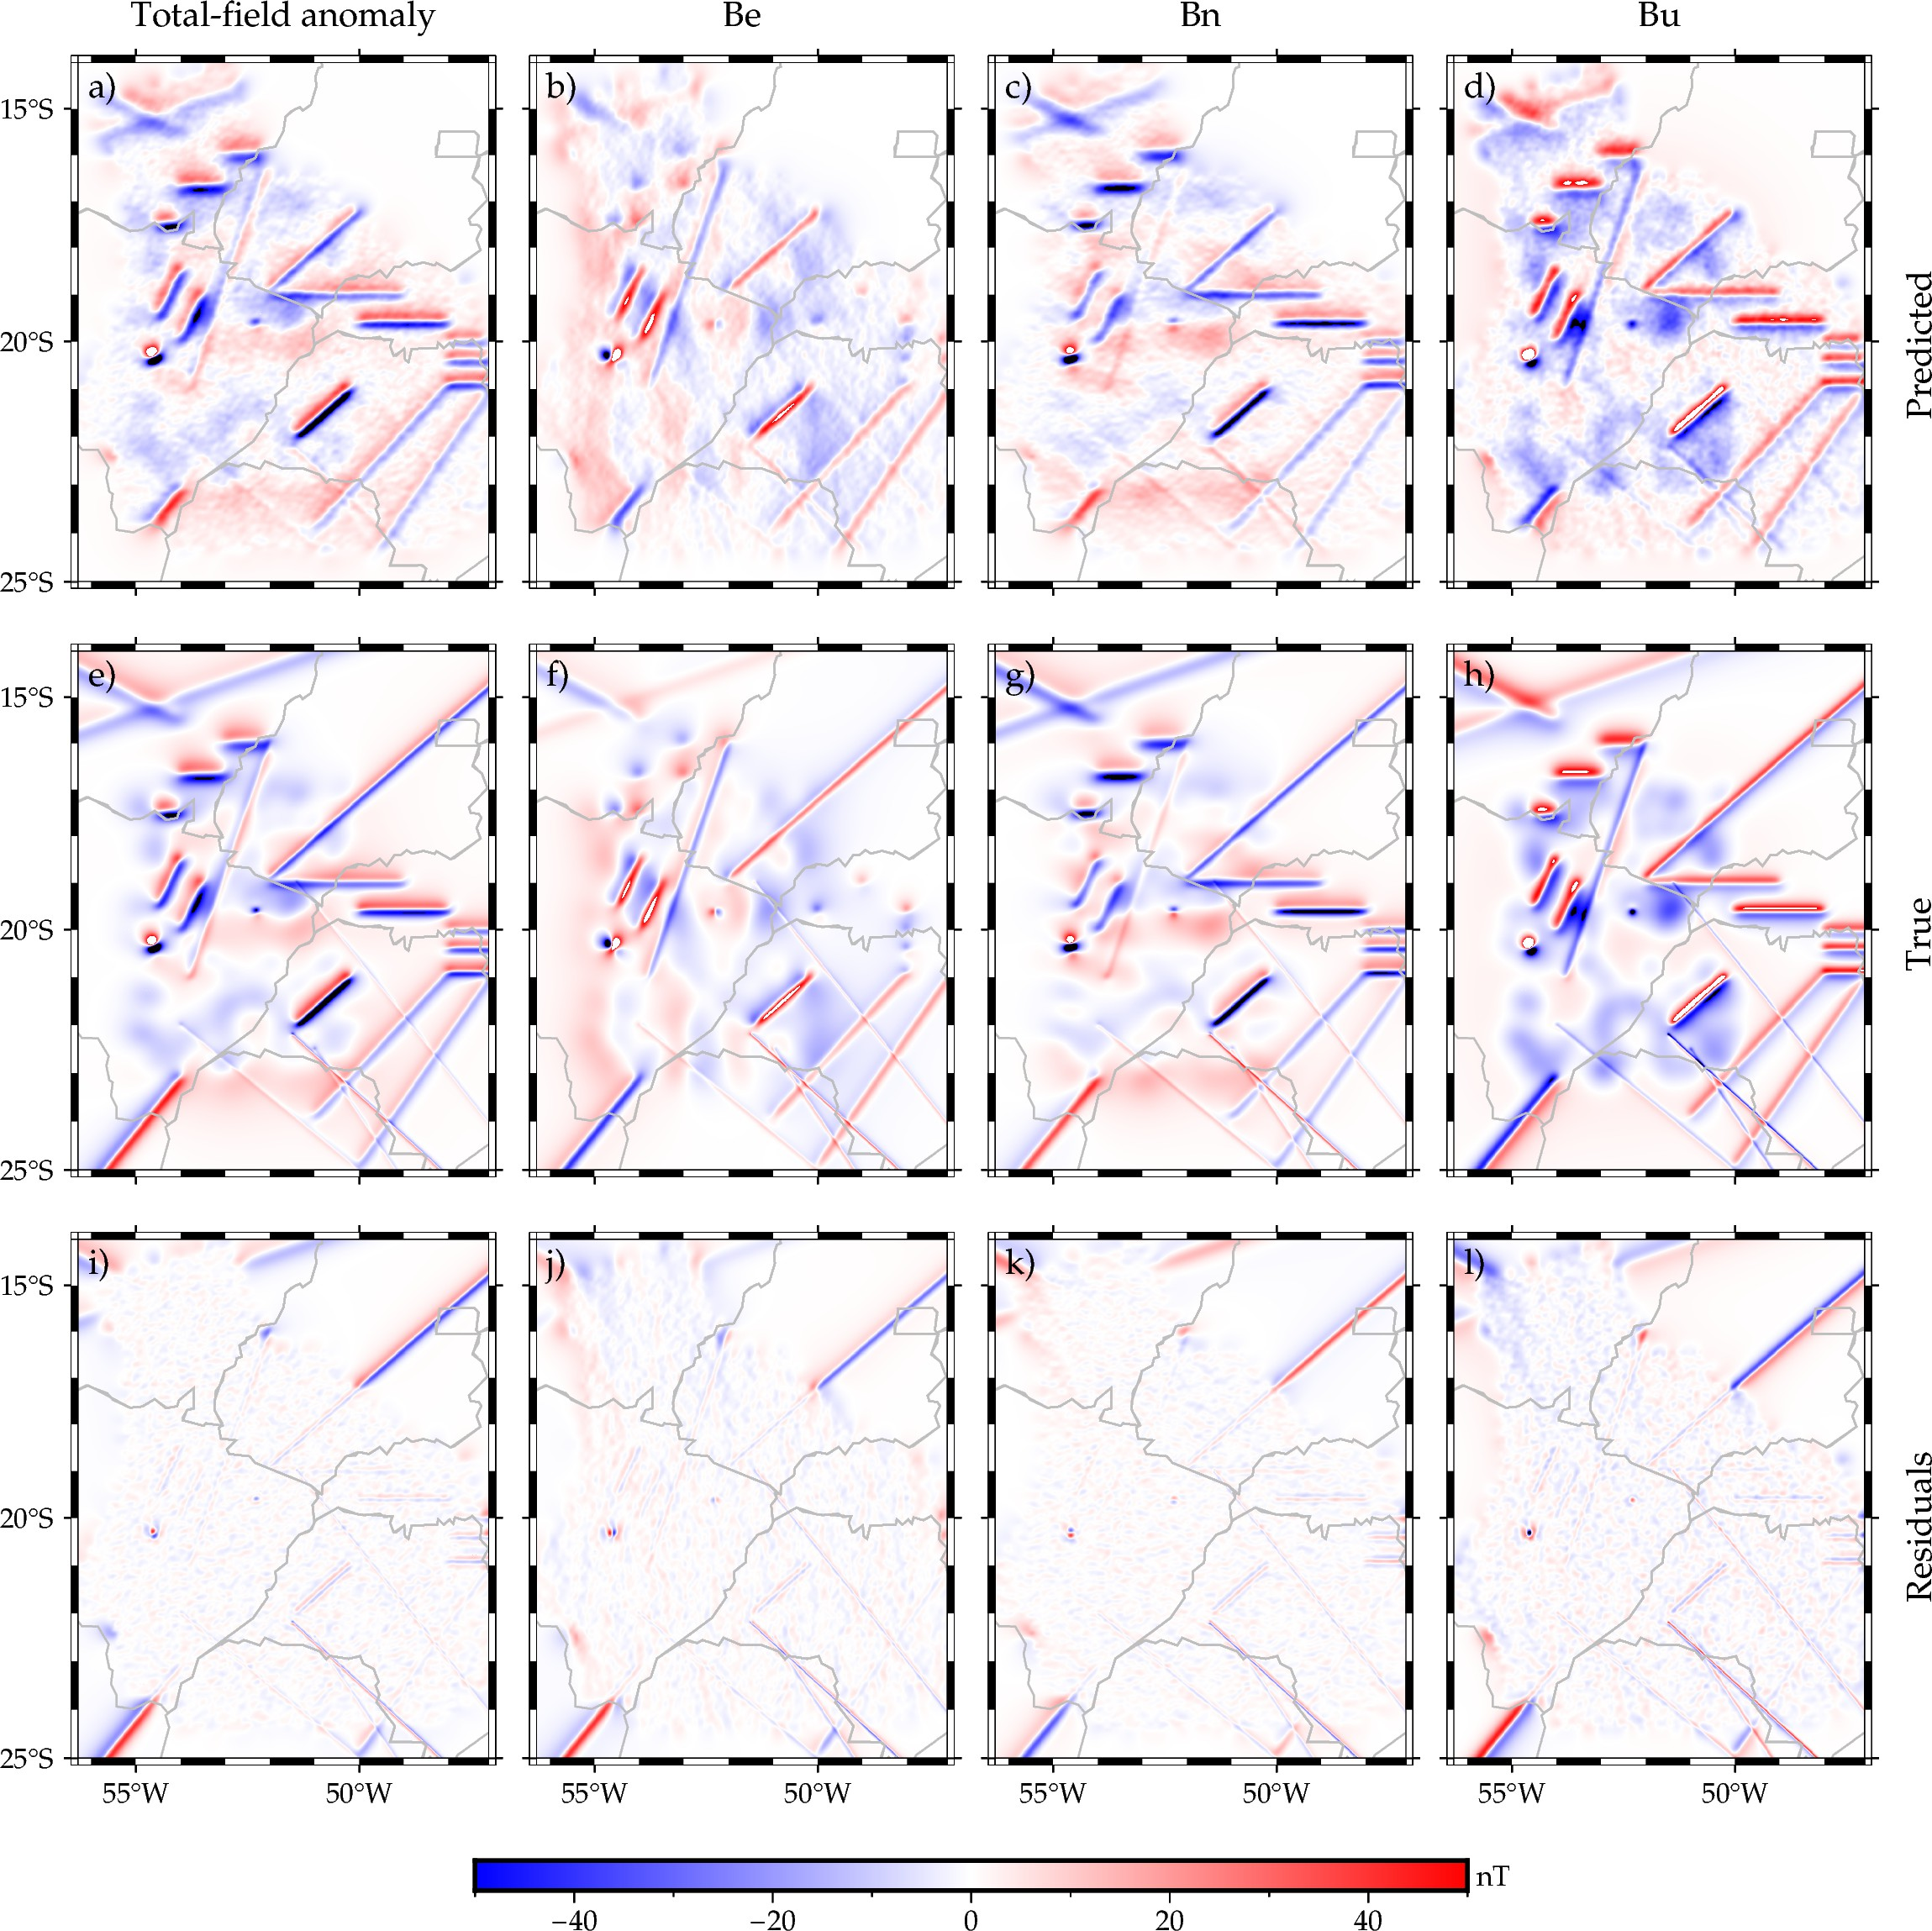
\includegraphics[width=1\linewidth]{figures/grided-TFA-B.jpeg}
% \caption{
%   \lipsum[1]
% }
% \label{fig_synthetic_simple_data}
% \end{figure}

\lipsum[5-10]


%%%%%%%%%%%%%%%%%%%%%%%%%%%%%%%%%%%%%%%%%%%%%%%%%%%%%%%%%%%%%%%%%%%%%%%%%%%%%%%
\section{Conclusion}

\lipsum[1-5]


%%%%%%%%%%%%%%%%%%%%%%%%%%%%%%%%%%%%%%%%%%%%%%%%%%%%%%%%%%%%%%%%%%%%%%%%%%%%%%%
\section{Open research}

The Python source code used to produce all results and figures presented here
is available at \url{https://github.com/\GitHubRepository} and
\url{https://doi.org/\ArchiveDOI} under the MIT open-source license.

Here we should cite all of the main software used, like Jupyter, numpy, scipy,
matplotlib, Fatiando, etc.

Cite any data sources as well.



%%%%%%%%%%%%%%%%%%%%%%%%%%%%%%%%%%%%%%%%%%%%%%%%%%%%%%%%%%%%%%%%%%%%%%%%%%%%%%%
\section{Acknowledgements}

We are indebted to the developers and maintainers of the open-source software
without which this work would not have been possible.
Acknowledge any non-author contributors to this study.
Statement about funding.

% Thank the editors and reviewers after review.